\documentclass{article}
\usepackage{tikz}

\begin{document}
    \begin{center}

        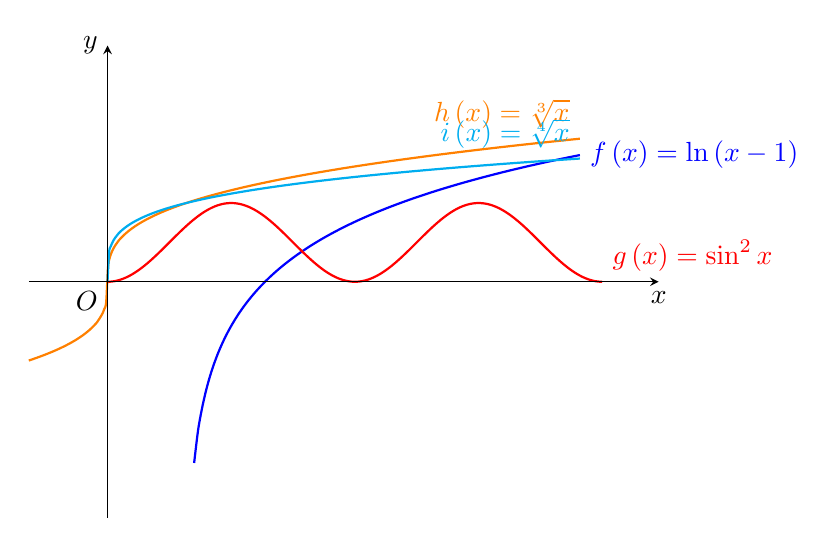
\begin{tikzpicture}
            %É necessário ter atenção aos domínios 
            %Df=]1,+inf[
            \draw[color=blue, thick, domain=1.1:6,smooth, samples=100] 
            plot (\x,{ln(-1+\x)}) node[right] {\(f\left(x\right)=\ln\left(x-1\right)\)};
            
            \draw[color=red, thick, domain=0:2*pi,smooth, samples=200] 
            plot ({\x},{(sin(\x r))^2}) node[above right] {\(g\left(x\right)=\sin^2 x\)};
    
            \draw[color=orange, thick, domain=-1:6,smooth,samples=300] 
            plot ({\x},{\x^(1/3)}) node[above left] {\(h\left(x\right)=\sqrt[3]{x}\)};
    
            %Di=[0,+inf[
            \draw[color=cyan, thick, domain=0:6,smooth,samples=300] 
            plot ({\x},{\x^(1/4)}) node[above left] {\(i\left(x\right)=\sqrt[4]{x}\)};

            \draw[->,>=stealth](-1,0) -- (7,0) node[below]{\(x\)};
            \draw[->,>=stealth](0,-3) -- (0,3) node[left]{\(y\)};
            \node at (0,0) [below left]{\(O\)};
        \end{tikzpicture}

        %Função paramétrica%

        \begin{tikzpicture}
            \draw[color=blue, thick, domain=0:2*pi,smooth,samples=300, variable=\p] 
            plot ({3*cos(\p r)},{2*sin(\p r)});

            \draw[->,>=stealth](-4,0) -- (4,0) node[below]{\(x\)};
            \draw[->,>=stealth](0,-3) -- (0,3) node[left]{\(y\)};
            \node at (0,0) [below left]{\(O\)};
        \end{tikzpicture}

        %Função polar
        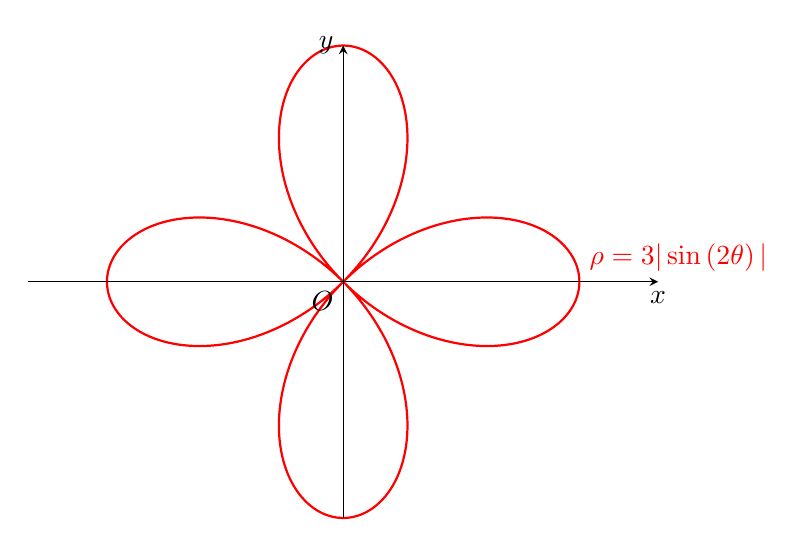
\begin{tikzpicture}
            \draw[color=red, thick, domain=0:360,smooth,samples=300, variable=\t] 
            plot ({\t}:{3*abs(cos(2*\t))}) node[above right]{\(\rho=3|\sin\left(2\theta\right)|\)};

            \draw[->,>=stealth](-4,0) -- (4,0) node[below]{\(x\)};
            \draw[->,>=stealth](0,-3) -- (0,3) node[left]{\(y\)};
            \node at (0,0) [below left]{\(O\)};
        \end{tikzpicture}

    \end{center}
\end{document}